% Two-column (vertical-flow) pipeline diagram for the poster.
% Standalone — compile with pdflatex, then rasterize for the poster panel.
% U-shape: read DOWN the left column, short hop at the bottom, then UP the right.
\documentclass[border=12pt]{standalone}
\usepackage{tikz}
\usepackage{amsmath}
\usetikzlibrary{shapes.geometric, arrows.meta, positioning}
\begin{document}
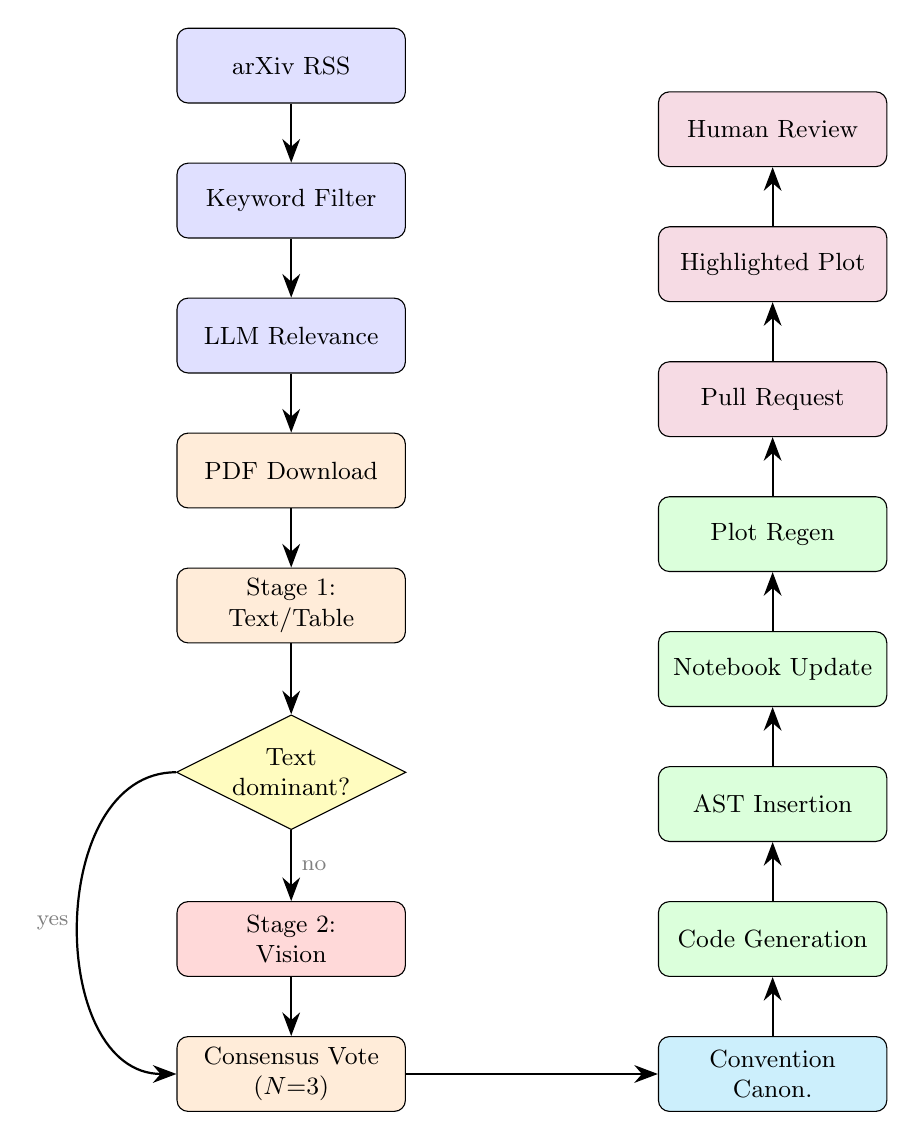
\begin{tikzpicture}[
    block/.style={rectangle, draw, rounded corners, minimum height=0.95cm,
                  minimum width=2.9cm, align=center, font=\small},
    decision/.style={diamond, draw, aspect=2, minimum width=2.0cm,
                     align=center, font=\small, inner sep=1pt},
    arrow/.style={-{Stealth[length=3mm]}, thick},
    lab/.style={font=\footnotesize, text=gray},
]

% ---------- Column 1: Discovery + Extraction (top -> bottom) ----------
\node[block, fill=blue!12]   (arxiv)                       {arXiv RSS};
\node[block, fill=blue!12,   below=0.75cm of arxiv] (kw)   {Keyword Filter};
\node[block, fill=blue!12,   below=0.75cm of kw]    (llm1) {LLM Relevance};
\node[block, fill=orange!15, below=0.75cm of llm1]  (pdf)  {PDF Download};
\node[block, fill=orange!15, below=0.75cm of pdf]   (text) {Stage 1:\\Text/Table};
\node[decision, fill=yellow!25, below=0.9cm of text] (check) {Text\\dominant?};
\node[block, fill=red!15,    below=0.9cm of check]  (vision){Stage 2:\\Vision};
\node[block, fill=orange!15, below=0.75cm of vision](vote) {Consensus Vote\\($N{=}3$)};

% ---------- Column 2: Convention + Integration + Review (bottom -> top) ----------
\node[block, fill=cyan!20,   right=3.2cm of vote]   (conv)    {Convention\\Canon.};
\node[block, fill=green!14,  above=0.75cm of conv]  (codegen) {Code Generation};
\node[block, fill=green!14,  above=0.75cm of codegen](ast)    {AST Insertion};
\node[block, fill=green!14,  above=0.75cm of ast]   (notebook){Notebook Update};
\node[block, fill=green!14,  above=0.75cm of notebook](plot)  {Plot Regen};
\node[block, fill=purple!14, above=0.75cm of plot]  (pr)      {Pull Request};
\node[block, fill=purple!14, above=0.75cm of pr]    (highlight){Highlighted Plot};
\node[block, fill=purple!14, above=0.75cm of highlight](human) {Human Review};

% ---------- Column 1 flow (down) ----------
\draw[arrow] (arxiv) -- (kw);
\draw[arrow] (kw)    -- (llm1);
\draw[arrow] (llm1)  -- (pdf);
\draw[arrow] (pdf)   -- (text);
\draw[arrow] (text)  -- (check);
\draw[arrow] (check) -- node[right, lab] {no} (vision);
\draw[arrow] (vision)-- (vote);
% "yes" bypass: arc on the LEFT, skipping the Vision box
\draw[arrow] (check.west) to[out=180, in=180, looseness=1.1]
      node[left, lab] {yes} (vote.west);

% ---------- Bottom hop: column 1 -> column 2 ----------
\draw[arrow] (vote) -- (conv);

% ---------- Column 2 flow (up) ----------
\draw[arrow] (conv)    -- (codegen);
\draw[arrow] (codegen) -- (ast);
\draw[arrow] (ast)     -- (notebook);
\draw[arrow] (notebook)-- (plot);
\draw[arrow] (plot)    -- (pr);
\draw[arrow] (pr)      -- (highlight);
\draw[arrow] (highlight)-- (human);

\end{tikzpicture}
\end{document}
